\documentclass[10pt]{article}

\makeatletter
\newcommand{\vast}{\bBigg@{3}}
\newcommand{\Vast}{\bBigg@{4}}
\makeatother

\usepackage{amsmath}
\usepackage{graphicx}
\usepackage[letterpaper]{geometry}
\usepackage{hyperref}

\setlength{\parindent}{20pt}
\setlength{\parskip}{8pt}
\graphicspath{ {./img/ }}

\author{James Randall}
\title{Catapult Construction and Modeling}

\begin{document}
\maketitle

%%%%%%%%%%%%%%%%
% Introduction %
%%%%%%%%%%%%%%%%

\begin{flushleft} 
\section{Introduction \& Purpose}
  This was something I'd been wanting to do for a while, so I just turned it in to a physics project.
  I built a catapult, and attempted to model the total launch distance of the projectile using the physics equations we've learned this year.
  So I created a bit of a lab out of it.
  The purpose of this lab is to model the launch distance of the catapult, given initial conditions (launch angle, spring constant, arm radius, etc...).
  I'm going to modify the typical lab structure slightly to make it more amenable to this project. 
  Instead of a background, I'm going to be covering all the math involved in Section IV.
  I'll knock out the "Final Project Essay" in Section II, and then in Section III I'll cover why I designed the catapult the ways that I did.
  Section IV will be the aforementioned derivation of the projectile distance projection, and section V will cover the experiment, assess how accurate the prediction was, sources of error, etc.  
  
  \par
  Also, there are several additions I've created to supplement this project. 
  \begin{itemize}
    \item \href{https://www.desmos.com/calculator/lioxjeyth8}{\underline{A Desmos visualization of the mathematical model I've created}} 
    \item \href{https://cad.onshape.com/documents/a21afbbb73f6dd6201e3b395/w/34e6c49428357ac916a3dcfd/e/86ecc9ec480ab3b6357f0414?renderMode=0&uiState=643624c739388d13bb3344de}{\underline{The CAD blueprint}}
    \item \href{https://imgur.com/a/iidlyPC}{\underline{A collection of images of the catapult, and screenshots of the CAD blueprint}} 
  \end{itemize}

%%%%%%%%%%%%%%%%%%%%%%%%%%%%%%%
% Applicable Physics Concepts %
%%%%%%%%%%%%%%%%%%%%%%%%%%%%%%%
  
\section{Applicable Physics Concepts}
  Math will not be discussed in this section.
  The equations will all be covered in section IV. For now, I'll just discuss relevant concepts for modelling the projectile distance.
  This project involves a little bit of almost everything we did this year. I'll cover the following:
  \begin{itemize}
    \item 2D Kinematics - Arc \& flight time of the projectile
    \item Hooke's Law and Tension - Catapult arm potential energy
    \item Rotational Motion - Catapult arm inertia, torque from tension
  \end{itemize}
  
  \subsection{2D Kinematics}
    Almost all of the math after the projectile leaves the catapult is modeled with 2D kinematics. 
    The projectile is in free fall, and the only force acting on the projectile is gravity 
    (Air resistance is neglected in the model).
    Once the launch angle of the projectile is found, the projectile's motion can be decomposed into its motion into two separte 1D kinematics equations.
    The vertical equation allows me to find the total airtime of the projectile, and because horizontal velocity is constant, this yields a total distance travelled for the projectile.

  \subsection{Hooke's Law}
    This will be covered more in Section III, but bungees are used bungees in order to apply torque to the catapult arm.  
    Hooke's law allows me to model the force applied by a bungee based on its displacement, because a bungee is literally just a spring.
    (This only works for displacement in the positive direction, because a bungee will just bend when it is compressed. 
    This does not occur with the catapult). 
    With some rotational motion physics and a pinch of calculus, we can use Hooke's law to find the launch velocity of the projectile. 

  \subsection{Rotational Motion}
    The catapult arm can be approximated as a line that moves around a fixed point, which meansthat the concepts we covered in our units on rotational motion are highly applicable.
    The tension in the bungees is a torque on the catapult arm, and we can use the moment of inertia for the catapult arm to find out the arm's angular acceleration.
    This ties in nicely with the previous subsection's discussion of Hooke's law, because as long as the angle between the arm and the bungee is known, we can determine the acceleration that the arm undergoes as the product of the bungee's force of tension.

%%%%%%%%%%%%%%%%%%%
% Catapult Design %
%%%%%%%%%%%%%%%%%%%

\section{Catapult Design}
  
  You can click \href{https://imgur.com/a/iidlyPC}{\underline{this link}} to view images of the catapult's CAD, and images of the catapult itself.
  Click \href{https://cad.onshape.com/documents/a21afbbb73f6dd6201e3b395/w/34e6c49428357ac916a3dcfd/e/86ecc9ec480ab3b6357f0414?renderMode=0&uiState=643624c739388d13bb3344de}{\underline{here}} to view and interact with the CAD model.
  The CAD model is the blueprint for the catapult, and some imperfections exist within the catapult that are not replicated in CAD.

  \subsection{Frame}
    The catapult base is 2ft $\cdot $ 3ft, and the entire frame is constructed out of 2x4 wood.
    The actual dimensions of a 2x4 are 1.5in and 3.5in respectively, so those are the width and height of every wooden component of the frame.

    \par
    The catapult's non-base section (referred to as the upper frame) consists of four diagonal pieces and a crossbar which runs between the diagonals.
    The diagonal pieces emerge from the base at a 45\textdegree \ angle, forming a right triangle when they meet.
    This was an intentional part of the design for two reasons:

    \begin{itemize}
      \item The crossbar can easily be attached to the diagonal pieces to yield a 45\textdegree \ launch angle
      \item Because the upper frame forms a right triangle, meaning that the angle between the arm and the bungees can be calculated easily as a function of the angle between the ground and the arm (This will be relevant in Section IV when dealing with torque).
    \end{itemize}

    In our unit on Kinematics, we learned that launching at 45\textdegree \ sends the projectile the farthest distance.
    In construction, the actual launch angle turned out to be 45\textdegree.
    This was accounted for in the subseqent calculations.
  
    % Catapult CAD Image
    \begin{figure}
      \caption{Isometric view of the catapult CAD model}
      \centering 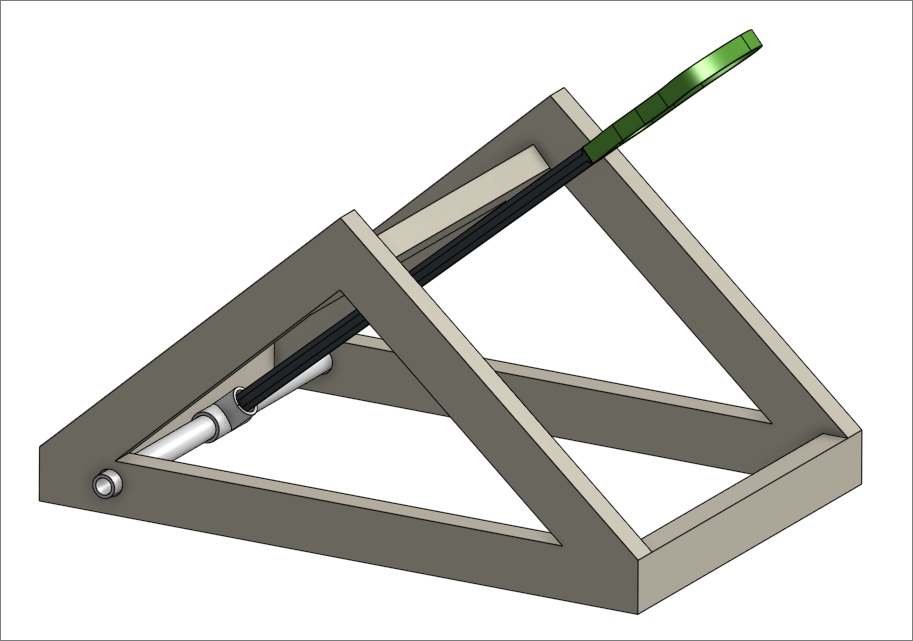
\includegraphics[width=5.0in, trim= 4 4 4 4, clip]{isometric}
    \end{figure}
  
  \subsection{Hinge}
    \par
    The arm's hinge is 1in PVC pipe, which has an outer diameter of 1.315in.
    In the base of the frame, a hole is drilled with a diameter of 1.317in, leaving just enough room to spin without friction.
    The hinge is placed at the front of the catapult.
    This is in contrast with traditional catapult designs.
    This choice was also made in order to achieve a 45\textdegree \ launch angle, and optimize launch distance.
    The PVC is ~26in in length (including the PVC Tee to attach the arm).
    The ends of the PVC that protrude from the frame are capped with PVC 1in endcaps to prevent the PVC from sliding out of the frame in operation.

  \subsection{Arm}
    \par
    The arm itself is comprised of a lacrosse stick and pvc pipe.
    It has a length of 36 inches.
    The bottom end is secured into a PVC pipe which connects to the PVC Tee and allows the arm to rotate around the hinge.
    Initially, the arm was facing forward and the open side of the net was facing downrange.
    After testing, the arm was flipped around, because it was determined that facing the stick forward caused friction on the projectile when the projectile was released. 
    This was because lacrosse sticks are meant for release at angles higher than 45\textdegree, so that the projectile can roll out of the top of the net.
    At 45\textdegree, the projectile does not do this. 
    This causes the projectile to roll along the bottom of the lacrosse stick's pocket, losing valuable linear velocity.
    To alleviate this, the stick was flipped backwards, so that the projectile can rest in the pocket but also does not lose as much energy on release.

  \subsection{Projectile}
    \par
    The projectile was purposefully selected to be as light as possible. 
    It's a golf ball. 
    This is because a lighter projectile would yield a more uniform moment of inertia for the catapult arm.
    If the projectile were disproportionately heavy, the estimated moment of inertia would be less accurate.
    Golf balls are also less prone to disruption by air resistance, because of the design of their surface and some other factors that are beyond the scope of this paper.
    Because the projectile is prone to bouncing and rolling after impact with the ground, it is advised to use the catapult on a flat surface of sand or gravel so that the first impact of the ball is visible. 
    This was the case in the experimental setup.

  \subsection{Bungees}
    \par
    The arm is attached to the upper frame via two bungees that run parallel to the crossbar.
    They are secured to zipties on the outside of the upper frame.
    In neutral position, the arm rests between the bungees and the crossbar.
    When the arm is pulled back, the bungees are stretched, and they form an isoceles triangle between the arm, and the two sides of the upper frame when viewed from the top. 

    \par
    The bungees are always slightly taught against the diagonal parts of the frame, meaning that as the arm is pulled back, the bungees travel in a straight line along the diagonal.
    This introduces some inaccuracy, because it means that the bungees are not attached to the arm at a fixed point.
    However, it makes the math much more simple to understand.

    \par
    When the arm is released, the bungees accelerate the arm, until it contacts the crossbar at which point it stops almost immediately.
    Before building the catapult, the spring coefficient of the bungees was determined to be 228 N/m.
    This was done by treating the two individual bungees as one, hanging a weight from both of them.
    The spring coefficient was then calculated using Hooke's law, because the weight of the hanging object as well as the bungee's displacement were known.
    Treating the two bungees as one spring makes the calculations in section IV easier.

%%%%%%%%%%%%
% The Math %
%%%%%%%%%%%%

  \section{The Math}

    This section will explain all of the physics equations used in order to predict how far the catapult will travel.
    Below are the variables, what they represent, and their units.
    More variables that are functions of ones listed below will be defined over the course of this section.
    
    \par
    This section will start with the variables defined in the first chart on the next page, and derive each of the variables in the second chart on the next page until the distance travelled is produced.
    This equation will take the form $x_1 = v_x0 \cdot t_a$ where $t_a$ is airtime.
    This means we must find the x component of the initial velocity, and the time in the air.

    \par
    Before reading this section, visit \href{https://www.desmos.com/calculator/lioxjeyth8}{\underline{this link}} to play around with a visual model in Desmos. 
    All parameters are modifiable, with the exception of the launch angle, because this would disrupt formulas that are dependent representing the upper frame as a right triangle.

    \begin{center}
      Chart of Fundamental Variables and Experimental Values
      \begin{tabular}{ |c|c|c|c| } 
        \hline
        Variable: & Value: & Units: & What it represents: \\ 
        $l_n$& 0.52 & m & The length at which the bungee has no potential energy \\ 
        $w$& 0.61 & m & The width of the catapult \\ 
        $k$& 219 & N/m & The spring constant of the bungee \\ 
        $\theta_0$& 8 & Deg & The angle to which the arm is pulled back \\ 
        $\theta_1$& 45 & Deg & The angle at which the projectile is released \\ 
        $r_o$& 0.6 & m & The length from the hinge that the bungees are attached \\ 
        $r_i$& 0.7 & m & The length from the hinge that the projectile sits \\ 
        $g$& 9.8 & m/s$^2$ & The acceleration due to gravity \\
        $m$& 0.36 & Kg & The mass of the catapult arm\\ 
        $l_a$& 0.99 & m & The length of the catapult arm\\ 
        \hline
      \end{tabular}
    \end{center}
    
    \begin{center}
      Chart of Nonintuitive Composite Variables \\
      \begin{tabular}{ |c|c|c| } 
        \hline
        Variable: & Units: & What it represents: \\ 
        $d_l$ & m & Linear distance between $r_i$ and the point of release \\
        $d_b$ & m & Total bungee displacement \\
        $F_T$ & N & Force of tension in the bungees \\
        $\alpha_1$ & Deg & Current catapult arm angle \\
        $\alpha_2$ & Deg & Angle between catapult arm and bungee\\
        $T_{avg}$ & N$\cdot$m & Average torque on catapult arm over launch period\\
        $a_{avg}$ & m/s$^2$ & Average acceleration of catapult arm over launch period\\
        $y_m$ & m & The maximum height that the projectile will reach\\
        $t_a$ & s & The total time that the projectile will spend in the air\\
        \hline
      \end{tabular}
    \end{center}

    \subsection{Finding the Initial Velocity}
    To find the initial velocity, we will take advantage of the fact that at the moment the projectile is released, all of its angular momentum is turned into linear momentum.
    Because the projectile's mass is constant, its angular velocity is therefore converted entirely into linear velocity.
    The remained of this subsection will be dedicated to finding the projectile's final angular velocity in the launch period.
    The first step is to define $\alpha_1$ that represents the current angle of the arm, and $d_l$ such that it represents the linear distance between the between the point at which the bungees are attached to the upper frame, and to the catapult arm.
    Therefore:
    
    $$d_l = r_i \cdot \sin(\theta_1 - a_1) $$
    
    In section III, it was mentioned that making the upper frame into a right angle made the math much more straightforward. This calculation is the reason for that. It means that we are able to use right-triangle trigonometry instead of the Law of Sines.
    (Keep in mind that the bungees travel in a straight line - they're constantly taught against the diagonal portions of the frame. This does mean that $r_i$ varies slightly, but it is a neglectable amount.)

    \par
    Once we have this angle, we can use this distance to find the total displacement of the bungees (reminder that $l_n$ is the neutral distance of the bungee, and $w$ is the catapult width).
    
    $$d_b = 2\sqrt{d_l^2 + \left( \frac{w}{2} \right)^2 } - l_n $$
    
    The radical is doubled because the pythoagorean theorem only gives the displacement for half of the bungee - the bungee and arm form two right triangles with the same hypotenuse, so we can find total displacement by doubling its half.
    We subtract $l_n$ to find the difference between the bungee's neutral and current length.

    \par
    A simple Hooke's Law application gives the force that the bungee exerts at this distance:
    $$ F_T = k \cdot d_b $$

    A quick detour will give us $a_2$, the angle between the arm and the bungee. Here we are taking advantage of the fact that all of the internal angles of a triangle add up to 180\textdegree, and that the upper frame forms a right triangle:
    
    $$\alpha_2 = \theta_1 + \alpha_1$$

    Another quick detour gives us the moment of inertia for the catapult arm, which is approximated as a uniform rod spinning about an end:

    $$I = \frac{1}{3} l_a m^2$$

    Now that we know the force and angle between the bungee and arm when the arm is at angle $a_1$, we can find the torque generated by the bungee at that angle.

    $$ T = r_1 F_T \cdot \sin(a_2) $$

    Remember that $F_T$ and $\alpha_2$ are functions of $\alpha_1$. 
    Therefore, if we find the average function value for T as $a_1$ goes from the inital to launch angle, we can account for the change in angle between the bungees and the arm, and also the change in force produced by the bungees:

    $$ T_{avg} = \frac{1}{\theta_1 - \theta_0} \int\limits_{\theta_0}^{\theta_1} T \mathrm{d} \alpha_1$$

    We can find the average acceleration on that same interval:

    $$ a_{avg} = \frac{T_{avg}}{I} $$
    
    And using our kinematics equations, we can find the angular velocity at time of release:

    $$\omega_0 = \cdot \sqrt{\frac{\pi (\theta_1 - \theta_0) a_{avg}}{90}}$$

    At this point, it's trivial to find the linear velocity. We just need to multiply the angular velocity by the catapult's projectile radius. We can also find the component velocities:
    
    $$ v_0 = r_o \cdot \omega_0  \ \ \ \ \ \ v_{x0} = \cos(\theta_1) \cdot v_0 \ \ \ \ \ \ v_{y0} = \sin(\theta_1) \cdot v_0 $$

    From this point forwards, it's just kinematics.

    \subsection{Finding the Airtime}

    This is the height of the projectile when it was launched:

    $$ y_0 = r_o \sin(\theta_1) $$

    And this is the equation to find the projectile's maximum height:

    $$ y_m = \frac{v_{y0}^2}{2g} + y_0 $$

    Once we have the maximum height, we can use it to find the total airtime:

    $$ t_a = \frac{v_{y0}}{g} + \sqrt{\frac{2y_m}{g}} $$

    And the total x displacement of the projectile is therefore:

    $$ x_1 = v_x0 \cdot t_a $$

    If you haven't already, visit the \href{https://www.desmos.com/calculator/xfx41esvkw}{\underline{Desmos simulation}} to get a better understanding of these mathematics.

    This is the equation we get if we refuse to define any new variables, and just substitute in the expressions using the fundamental variables of the catapult.
    I know it looks disgusting, but it was so much worse before I simplified it.

\end{flushleft}

%%%%%%%%%%%%%%%%%%%%%%%%%%%%%%%%%%%%%%%%%%%%
% The Really Big Hairy Nasty Ugly Equation %
%%%%%%%%%%%%%%%%%%%%%%%%%%%%%%%%%%%%%%%%%%%%  

  \center{The Really Big Hairy Nasty Ugly Equation}
  \begin{equation*}
    \begin{gathered}
      % Chunk One:
      x_d = 
      \frac { r_o \cos(\theta_1) } {gl_a} 
      \vast[
        \frac{\pi r_o}{30ml_a} 
        \int\limits_{\theta_0}^{\theta_1} 
          kr_i \left( 2
            \sqrt{
              (r_i sin (\theta_1 - a_1))^2
              + \frac{w^2}{4}
            } - l_n 
          \right)
          \sin(\theta_1 + a_1) 
        \mathrm{d}a_1
        \sin(\theta_1) \
      \\
      % Chunk Two: 
      + \begin{gathered} 
        \sqrt{ 
          \frac{\pi}{30m} 
          \int\limits_{\theta_0}^{\theta_1}
            kr_i \left( 2 
              \sqrt{
                (r_i sin (\theta_1 - a_1))^2
                + \frac{w^2}{4}
              } - l_n
            \right) 
            \sin(\theta_1 + a_1) 
          \mathrm{d}a_1 } 
      \end{gathered}
      \ \cdot
      \\
      % Chunk Three:
      \begin{gathered}
        \sqrt{
          \begin{gathered} 
              \frac{\pi r_o^2}{30ml_a^2} 
              \int\limits_{\theta_0}^{\theta_1}
                kr_i \left( 2 
                \sqrt{
                  (r_i sin (\theta_1 - a_1))^2
                  + \frac{w^2}{4}
                } - l_n
                \right) \sin(\theta_1 + a_1) \mathrm{d}a_1  \sin^2(\theta_1) 
          \end{gathered} 
        + 2gr_o \sin(\theta_1) } \ 
      \end{gathered} \vast]
    \end{gathered}
    \strut
  \end{equation*}

  \begin{flushleft}
  \section{The Science}
    
    The purpose of this section is to examine how closely the real catapult aligns with the predictions made by the model created in Section IV. 
    It will be similar to an in-class lab, sans the purpose and background, because they have already been established in previous sections.
    
    \subsection{Materials}
      \begin{enumerate}
        \item Catapult
        \item Golf ball
        \item Measuring tape
        \item Flat surface of sand or gravel
      \end{enumerate} 

    \subsection{Procedure}
      \begin{enumerate}
        \item Set up the catapult on a surface of gravel or sand
        \item Load the projectile into the catapult arm
        \item Pull the catapult arm back to the maximum possible displacement
        \item Release the catapult arm
        \item Measure the distance between the center of the catapult and the projectile's first bounce
        \item Repeat steps 1-5 at least 5 times
      \end{enumerate}

    \subsection{Data}   
    
      \begin{center}
      \begin{tabular}{ |c|c|c|c|c|c|c| } 
       \hline
             Trial \#: & Trial 1 & Trial 2 & Trial 3 & Trial 4 & Trial 5 & Average \\ 
             Distance (m): & 13.82 & 15.67 & 14.94 & 15.19 & 14.71 & 14.87 \\ 
       \hline
      \end{tabular}
      \end{center}

      Plugging the experiment's conditions into the model derived in section IV gives a theoretical distance of 15.54 meters.

      \par 
      Percent Error is therefore:
      $$ \left| \frac{14.87 - 15.54}{15.54} \right| \cdot 100\% = 4.3\% $$

    \subsection{Sources of Error}
      There are several large sources of error in this experiment:
      \begin{itemize}
        \item In the equations, it was assumed that the bungees were always attached to the arm at a fixed point. 
          This was not the case. 
          They were allowed to slide up and down the arm as it rotated so that the bungees would travel in a straight line.
          This meant that the value of $r_i$ in the math varied by about 0.03 over the course of the launch period.
        \item The bungees have a slight tension in the neutral position, meaning that the bungee's displacement never actually reaches 0, and is offset by a positive constant during the launch period.
        \item Air resistance was not factored in to the prediction. 
          This would potentially decrease the actual travel distance of the ball, and lead to discrepancies between the catapult and the model.
          Although golf balls are less prone to air resistance, it is still not a factor that can be ignored.
      \end{itemize}

    \subsection{Conclusion}
      This model was significantly more accurate than was expected. Originally there were several errors in the equation, leading to a percent error of approximately 20\%. Tweaking the model has made it an accurate prediction of the horizontal launch distance of the catapult.

\end{flushleft}
\end{document}
